\documentclass[a4paper, 12pt, notitlepage]{report}
\raggedbottom
\sloppy
\clubpenalty1000%
\widowpenalty1000%
\renewcommand{\baselinestretch}{1.1}

\usepackage[english]{babel}
\usepackage[pdftex,unicode]{hyperref}
\usepackage{helvet}
\usepackage{graphicx}
\usepackage{colortbl}
\date{}

\newcommand{\xsversion}{PRODUCT}
\newcommand{\refversion}{REFERENCE}

\title{Performance Report\\\vspace{10mm}\xsversion\\vs\\\refversion}

\begin{document}

\maketitle

\chapter* {Summary}

\section*{Overview}

\input{summary.tex}

\subsection*{Magnitude of Results}

\begin{figure}[h]
\centering
\includegraphics[width=0.6\textwidth]{PATH/bettercount.pdf}
\caption{Cumulative Frequency of Performance Improvement Magnitudes}
\end{figure}

\begin{figure}[h]
\centering
\includegraphics[width=0.6\textwidth]{PATH/worsecount.pdf}
\caption{Cumulative Frequency of Performance Loss Magnitudes}
\end{figure}

\section*{Comments}

The first thing to note is that the use of 'significant' in the overview above is in
the sense of 'statistically' rather than 'considerable'.
 


\newpage

\tableofcontents

\newpage

\chapter {Interpreting the Graphs}

\section{Forest Plots}

\begin{figure}[h]
\centering
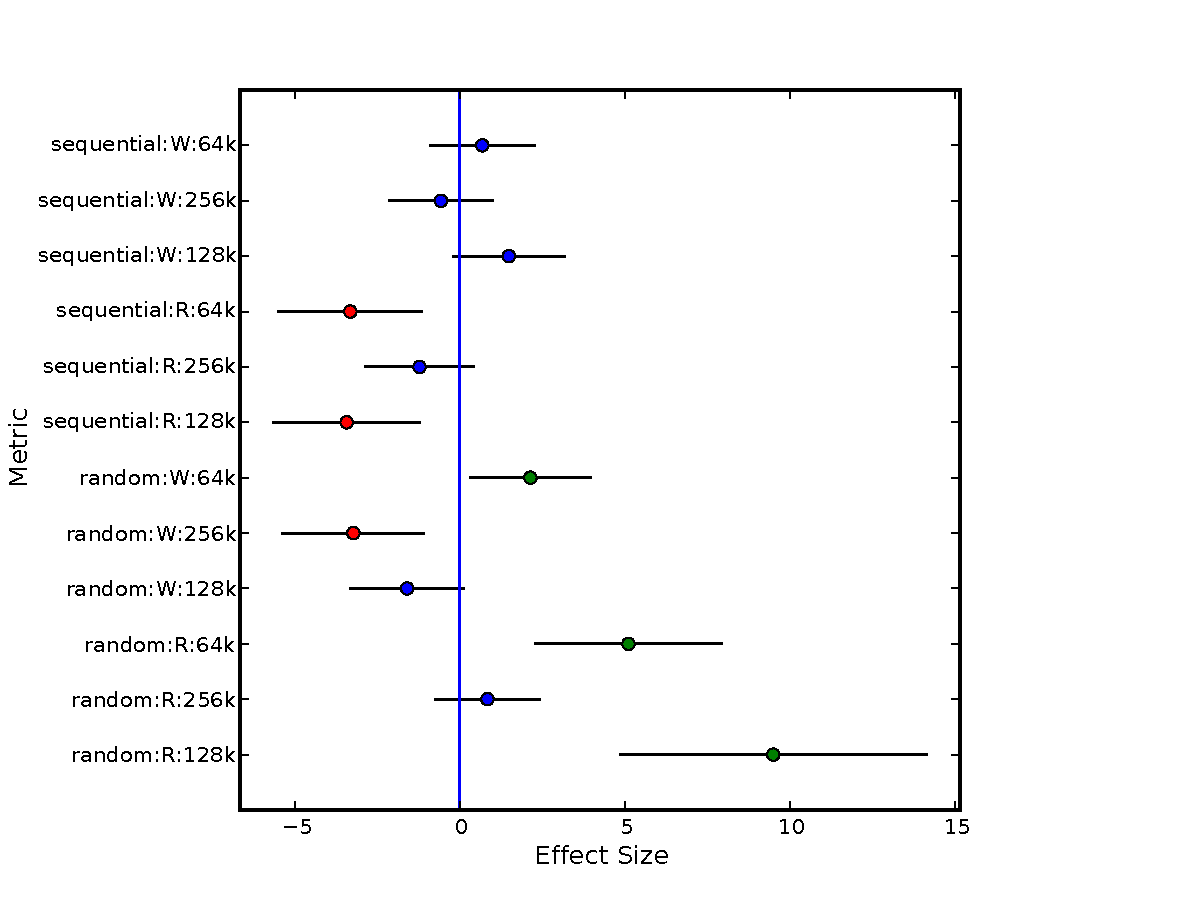
\includegraphics[width=0.6\textwidth]{PATH/forestexample.pdf}
\caption{Example Forest Plot}
\end{figure}

A forest plot is a plot of effect size and confidence interval against metric.
They are used to plot the results of benchmarks that have a large number of 
metrics. Effect size is the mean difference observed between product and 
reference measurements divided by the pooled standard deviation of all the 
measurements. The confidence intervals shown by the horizontal black lines 
are the ranges into which the actual effect size is 95\% likely to fall.  
If this range crosses zero the result is insignificant. Significant 
improvements in performance are shown as green circles, significant 
performance losses as red circles and insignificant results as blue circles. 

\section{Bar Charts}

\begin{figure}[h]
\centering
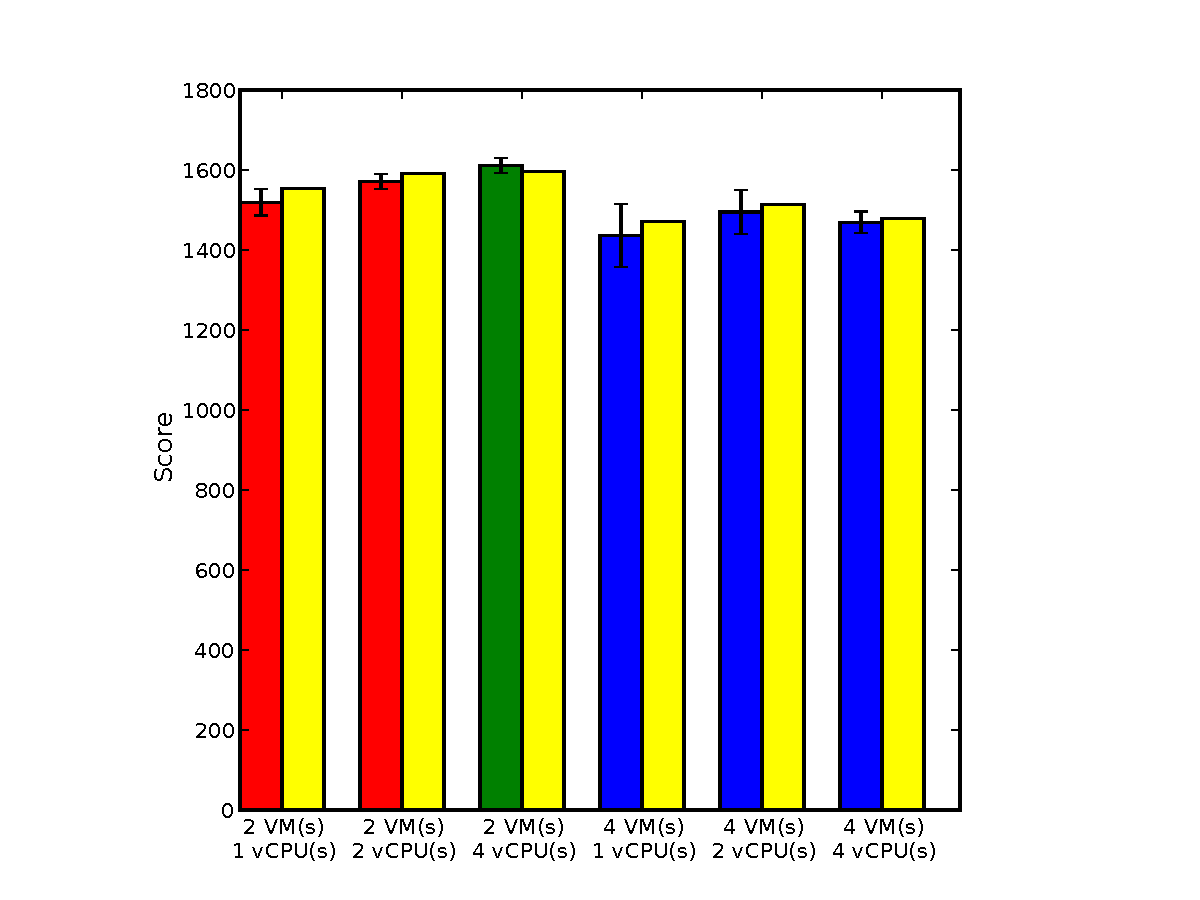
\includegraphics[width=0.6\textwidth]{PATH/barexample.pdf}
\caption{Example Bar Chart}
\end{figure}

A bar chart is used to plot test configuration against test result for 
benchmarks with a small number of metrics. Each pair of bars shows the
mean product result against the mean reference result. The product bar 
may be coloured red, green or blue depending on if the result is 
significantly worse, significantly better or insignificant respectively.
The reference bar is always coloured yellow. Error bars on the product
bar show the range in which it is 95\% likely that the true mean will fall.
If the error bars overlap the reference mean then the result is insignificant.

\section{Tables}

Each graph is accompanied by a data table. For each bar or effect size plotted
the table shows the actual mean product result, the number of product results,
mean reference result, the number of reference results and 
percentage difference between the two. The rows of the table are coloured
according to if the results are significantly better (green), significantly
 worse (red) or insignificant (white).

\newpage

\chapter {Results}

\input{PATH/data.tex}

\end{document}
